\documentclass[12pt]{article}
\usepackage{amsmath}
\usepackage{amsfonts}
\usepackage{amssymb}
\usepackage{amsthm}
\usepackage[top=1in, bottom=1in, left=1in, right=1in]{geometry}
\usepackage{tikz}
\usetikzlibrary{automata,topaths,arrows}
\usepackage{caption}
\usepackage{graphicx}
\usepackage{float}
\usepackage{alltt}
\usepackage{mathrsfs}
\usepackage{ulem}
\usepackage{verbatim}

\newtheorem{theorem}{Theorem}[section]
\newtheorem{corollary}{Corollary}[theorem]

\theoremstyle{definition}
\newtheorem{defn}{Definition}[section]

\theoremstyle{remark}
\newtheorem*{remark}{Remark}

\newcommand\Tau{\mathrm{T}}
\newcommand\sgn{\text{sgn}}

\newcommand{\bbR}{\mathbb{R}} %shorter commands for ``Blackboard Bold" letters
\newcommand{\bbZ}{\mathbb{Z}}
\newcommand{\bbN}{\mathbb{N}}
\newcommand{\bbC}{\mathbb{C}}
\newcommand{\bbQ}{\mathbb{Q}}
\newcommand{\bbP}{\mathbb{P}}
\begin{document}

Throughout this paper we will refer to a fixed regulatory network $\textnormal{\textbf{RN}} = (V,E)$ with network nodes $V = \{x_1,x_2,\dots,x_n\}$ and interactions $E \subset V \times V \times \{\rightarrow,\dashv\}$. We define the \textit{targets} of a node as
\begin{equation*}
\mathbf{T}(x_i):=\{x_j \mid (x_i,x_j) \in \mathbf{RN} \}
\end{equation*}
and the \textit{sources} of a node as 
\begin{equation*}
\mathbf{S}(x_i):=\{x_j \mid (x_j,x_i) \in \mathbf{RN} \}
\end{equation*}

\section{General System}
We define a general system of \textbf{RN} as 
\begin{equation}	\label{generalsystem}
\dot{x}_j=-\gamma_j x_j + \sum_{I\in \mathcal{I}}\left(\prod_{i\in I}\sigma_{ji}(x_i)\right)	\qquad	j=1,\dots,n
\end{equation}
where $\mathcal{I}\subseteq \mathscr{P} \{1,\dots,n\}$ and $\sigma_{ji}(x_i)$  is a linear ramp defined if $(x_i,x_j) \in E$ as
\begin{equation}	\label{sigma}
\sigma_{ji}(x_i):=
\begin{cases}
l_{ji}	&	\text{for } x_i \le \theta_{ji}-\frac{\epsilon}{2}\ \text{and } x_i\to x_j, \text{or } x_i\geq\theta_{ji}+\frac{\epsilon}{2} \text{ and } x_i\dashv x_j\\
u_{ji}	&	\text{for}\ x_i \geq\theta_{ji}+\frac{\epsilon}{2}\ \text{and}\ x_i\dashv x_j, \text{or}\ x_i\le\theta_{ji}-\frac{\epsilon}{2} \text{ and } x_i\to x_j\\
+\frac{u_{ji}-l_{ji}}{\epsilon}(x_i-\theta_{ji}) + \frac{u_{ji}+l_{ji}}{2} &  \text{for } \theta_{ji}-\frac{\epsilon}{2}<x_i<\theta_{ji}+\frac{\epsilon}{2} \text{ and } x_i\to x_j\\
-\frac{u_{ji}-l_{ji}}{\epsilon}(x_i-\theta_{ji}) + \frac{u_{ji}+l_{ji}}{2} & \text{for } \theta_{ji}-\frac{\epsilon}{2}<x_i<\theta_{ji}+\frac{\epsilon}{2} \text{ and } x_i\dashv x_j\\
\end{cases}
\end{equation}	

The constants $u_{ji}$ and $l_{ji}$  and the thresholds $\theta_{ji}$ are as previously defined. The constant $\epsilon$ is introduced for all $\sigma_{ji}(x_i)$ such that $\epsilon>0$ and $\epsilon$ is small enough to satisfy $\theta_{ki}-\frac{\epsilon}{2},\theta_{ki}+\frac{\epsilon}{2}\notin [\theta_{ji}-\frac{\epsilon}{2},\theta_{ji}+\frac{\epsilon}{2}]$ for any $i,j,k$ with $j \neq k$. That is, no epsilon bands overlap, and so for any particular value of $x_i$, at most only one $\sigma_{ji}(x_i)$, where $x_j\in\mathbf{T}(x_i)$, is in its linear region. Therefore, we can classify intervals of $x_i$ as two distinct types.

\begin{figure}[h]	\label{sigmagraph}
\centering
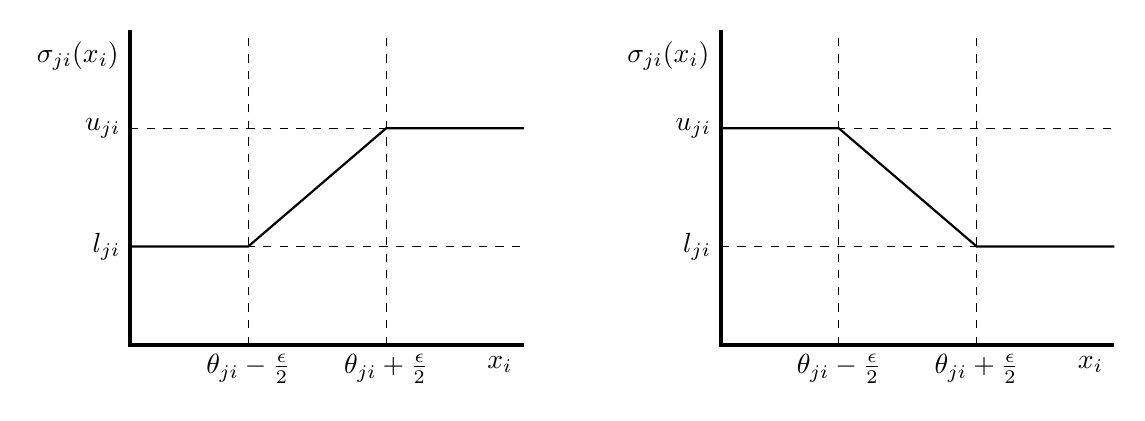
\begin{tikzpicture}[scale=1]
%\draw[step=.5cm,grey,very thin] (0,0) grid (5,4);
\draw[ultra thick] (0,4) node[anchor=north east]{$\sigma_{ji}(x_i)$} -- (0,0) -- (5,0) node[anchor=north east]{$x_i$} ;
\draw[thick] (0,1.25) -- ++(1.5,0) -- ++(1.75,1.5) -- ++(1.75,0);

\draw[dashed] (1.5,0) node [below]{$\theta_{ji}-\frac{\epsilon}{2}$} -- ++(0,4);
\draw[dashed] (3.25,0) node [below]{$\theta_{ji}+\frac{\epsilon}{2}$} -- ++(0,4);

\draw[dashed] (0,1.25) node[anchor=east]{$l_{ji}$} -- ++(5,0);
\draw[dashed] (0,2.75) node[anchor=east]{$u_{ji}$}-- ++(5,0);

\draw[ultra thick] (7.5,4) node[anchor=north east]{$\sigma_{ji}(x_i)$} -- (7.5,0) -- (12.5,0) node[anchor=north east]{$x_i$} ;
\draw[thick] (7.5,2.75) -- ++(1.5,0) -- ++(1.75,-1.5) -- ++(1.75,0);

\draw[dashed] (9,0) node [below]{$\theta_{ji}-\frac{\epsilon}{2}$} -- ++(0,4);
\draw[dashed] (10.75,0) node [below]{$\theta_{ji}+\frac{\epsilon}{2}$} -- ++(0,4);

\draw[dashed] (7.5,1.25) node[anchor=east]{$l_{ji}$} -- ++(5,0);
\draw[dashed] (7.5,2.75) node[anchor=east]{$u_{ji}$}-- ++(5,0);

\end{tikzpicture}
\caption{Left: A graph of $\sigma_{ji}(x_i)$ versus $x_i$ if $x_i \to x_j$. Right: The graph if $x_i \dashv x_j$.}
\end{figure}

\begin{defn}	\label{IntervalType}
We define a closed interval of $x_i$, denoted $I_{R,i}$, as \textit{Type R}, i.e. in a particular linear ramp region, if $\exists x_j\in\mathbf{T}(x_i)$ with associated thresholds $\theta_{ji}-\frac{\epsilon}{2},\theta_{ji}+\frac{\epsilon}{2}$ such that $I_{R,i}=\left[\theta_{ji}-\frac{\epsilon}{2},\theta_{ji}+\frac{\epsilon}{2}\right]$ for some $x_j \in \mathbf{T}(x_i)$.

We define a closed interval of $x_i$, denoted $I_{C,i}$, as \textit{Type C} if $\exists x_q,x_r \in \mathbf{T}(x_i)$ with $q\neq r$ and $\theta_{qi}+\frac{\epsilon}{2}<\theta_{ri}-\frac{\epsilon}{2}$ such that $I_{c,i}:=[\theta_{qi}+\frac{\epsilon}{2},\theta_{ri}-\frac{\epsilon}{2}]$ or $I_{c,i}:=(-\infty,\theta_{qi}-\frac{\epsilon}{2}]$ or $I_{c,i}:=[\theta_{ri}+\frac{\epsilon}{2},\infty)$ and there is no Type R interval $I_{R,i}$ such that $I_{R,i}\subset I_{C,i}$. 
\end{defn}

{\color{cyan} Peter: I'd like to get rid of the infinities as endpoints of the Type C intervals. Bree mentioned something about compact metric spaces or something of the like. Could that be used?}

\begin{remark}
From Definition \ref{IntervalType}, note that every Type R interval is connected to two Type C intervals.
\end{remark}

\begin{defn} \label{kappa}
 We divide phase space into \textit{cells}, denoted $\kappa$. We define $\kappa$ as the product of the closed intervals
 \begin{equation}	\label{kappadefn}
 \kappa:=\prod_{i=1}^n I_{*,i} \quad \text{ where } \quad *=
 \begin{cases} 
 C & \text { if } i\in\alpha_c \\
 R & \text{ if } i \in \alpha_R
 \end{cases}
 \end{equation}
 where $\alpha_R$ and $\alpha_C$ partition $\{1,\dots,n\}$. We label $\kappa$ a  $m$-cell, where $m$ is the cardinality of $\alpha_R$, because in $\kappa$, there are $m$ equations of system \eqref{generalsystem} that are in their linear ramp section.

We defined two cells $\kappa$ and $\kappa'$ as adjacent if 
\begin{equation*}
\kappa:=\prod_{i=1}^n I_{*,i} \quad \text{ where } \quad *=
 \begin{cases} 
 C & \text { if } i\in\alpha_C \\
 R & \text{ if } i \in \alpha_R
 \end{cases}
 \end{equation*}
 and 
 \begin{equation*}
\kappa':=\prod_{i=1}^n I_{*',i} \quad \text{ where } \quad *'=
 \begin{cases} 
 C & \text { if } i\in\alpha_C' \\
 R & \text{ if } i \in \alpha_R'
 \end{cases}
 \end{equation*}
 where $\alpha_R$ and $\alpha_C$ partition $\{1,\dots,n\}$ and there exists some $k\in \{1,\dots,n\}$ such that $\alpha_C'=\alpha_C\setminus \{k\}$ and $\alpha_R'=\alpha_R\cup \{k\}$, and $I_{C,k}$ and $I_{R,k}$ are adjacent intervals. Then $\kappa'$ is an $(m+1)$-cell, where $m$ is the cardinality of $\alpha_R$.
 
We define the $n-1$ dimensional hyperplane $\kappa \cap \kappa'$ as the \textit{wall} between cells $\kappa$ and $\kappa'$ as the product
\begin{equation*}
\tau:=\prod_{i=1}^{k-1} I_{*,i} \times \{\vartheta_k\} \times \prod_{i=k+1}^{n} I_{*,i}
\end{equation*}
where $\vartheta_k = \theta_{jk} \pm \frac{\epsilon}{2}$ for some $j$. We refer to $\tau$ as a wall of the $m$-cell $\kappa$.
\end{defn}

\begin{remark}
It is worth noting that all cells and walls are closed. Also, note that we use $\theta_{ji}+\frac{\epsilon}{2}$, with two subscripts, to denote a threshold of system \eqref{generalsystem}, and $\vartheta_k$, with one subscript, to denote some constant that is the endpoint of some interval of $x_k$.
\end{remark}

\begin{defn}
Let $\kappa$ be some cell of $\bbR^n$ with associated $\alpha_R$ and $\alpha_C$. From Definition \ref{IntervalType}, for each $i\in\alpha_R$ and corresponding $I_{R,i}$, let $r_i^+$ and $r_i^-$ be constants such that $I_{R,i}=[r_i^-,r_i^+]$, and for each $i\in\alpha_C$ and corresponding $I_{R,i}$, let $c_i^+$ and $c_i^-$ be constants such that if $I=[\theta_{qi}+\frac{\epsilon}{2},\theta_{ri}-\frac{\epsilon}{2}]$ then $I_{C,i}=[c_i^-,c_i^+]$, or {\color{cyan} Dissipative System here} . Let $P_i$ be the set defined as 
\begin{equation*}
P_i :=
\begin{cases}
\{r_i^-,r_i^+\} &  \text{ if } i\in \alpha_R \\
\{c_i^-,c_i^+\} &  \text{ if } i\in \alpha_C \\
\end{cases}
\end{equation*}
We define the set of \textit{corner points} of a cell $\kappa$, denoted $\bbP(\kappa)$, as the product of sets 
\begin{equation*}
\bbP (\kappa) := \prod_{i=1}^n P_i
\end{equation*}
Notice that the cardinality of $\bbP (\kappa)$ is $2^n$. Let $p_1,\dots,p_{2^n}$ be the elements of $\bbP (\kappa)$.
\end{defn}

\begin{defn} \label{flowDefn}
Suppose $H$ is some subset of a co-dimension $n-1$ hyperplane with normal vector $\vec{h}$ and suppose a vector $\dot{x}(P)$ such that $\dot{x}(P)=\langle \dot{x}_1(P),\dots,\dot{x}_n(P) \rangle$ where $\dot{x}_j(P)$ denotes $\dot{x}_j$ evaluated at some point $P$. We define the \textit{flow} of system \eqref{generalsystem} to be \textit{monotonic} in the direction of $\vec{h}$ on $H$ if $\forall$ points $P$ such that $P\in H$, $\vec{h}\cdot\vec{x}(P)>0$, and monotonic in the direction of $-\vec{h}$ on $H$ if $\forall$ points $P$ such that $P\in H$, $\vec{h}\cdot\vec{x}(P)<0$. 
We define the flow to be bidirectional across $H$ if $\exists$ points $P_1,P_2$ such that $P_1,P_2 \in H$, $\vec{h}\cdot\vec{x}(P_1)>0$ and $\vec{h}\cdot\vec{x}(P_2)<0$.
\end{defn}

\begin{defn} \label{sgnDefn}
Let $A$ be any closed bounded region of $\bbR^n$, and let $P$ and $P'$ be points.  We introduce the function $\sgn(A,k)$ to classify the behavior of the solutions to system \eqref{generalsystem} in $A$, defined as 
\begin{equation}
\sgn(A,k)=
\begin{cases}
+1	&	\text{if } \forall P\in A, \dot x_k (P)>0\\
-1	&	\text{if } \forall P\in A, \dot x_k (P)<0\\
0	&	\text{if } \exists P,P'\in A \text{ such that }  \dot x_k (P)>0 \text{ and } \dot x_k (P')<0\\
\end{cases}
\end{equation}
\end{defn}

\begin{remark}
From Definitions \ref{flowDefn} and \ref{sgnDefn} that if $\tau$ is some wall in $\mathbb{R}^n$ such that $\tau \subseteq \{x_k=\vartheta_k\}$, then $\sgn(\tau,k)=+1$ implies that the flow is monotonic in the $\vec e_k$ direction across $\tau$, and similarly $\sgn(\tau,k)=-1$ implies that the flow is monotonic in the $-\vec e_k$ direction across $\tau$. We will use this fact to construct the domain graph of system \eqref{generalsystem}.
\end{remark}

{\color{cyan} Peter: The next theorem and proof is incomplete, but I'll probably leave the proof to Thomas or Bree. The Generic proof argument still escapes me.}

\begin{theorem}
Suppose $\kappa$ is a  $0$-cell, and $\tau$ is a face of $\kappa$. It is generic that $\sgn(\tau)\neq 0$.
\end{theorem}

\begin{proof}
Let $\tau\subseteq \{x_k=\vartheta_k\}$. Then $\vec{e}_k\perp \tau$ By definition of  $0$-cell, $\kappa$ is the product of n Type C intervals, and so all $\sigma_{ki}(x_i)$ are constants. The $k^\text{th}$ equation of system \eqref{generalsystem} can then be written as $\dot x_k=-\gamma_kx_k+C_k$, where $C_k$ is some constant. On $\tau$, $x_k=\vartheta_k$, and so by substitution, $\dot x_k = -\gamma_k \vartheta_k + C_k$ on $\tau$. Therefore, $\dot{x}_k=0$ only if $\gamma_k\vartheta_k=C_k$. Otherwise, $\dot{x}_k$ is some non-zero constant, and so by Definition \ref{sgnDefn}, $\sgn(\tau)\neq 0$.
\end{proof}

{\color{cyan} Peter: The next theorem is the straight-line proof. I've completely rewritten it to be much more general.}

\begin{theorem} \label{straightlineproof}
Suppose $\kappa$ is some cell in $\mathbb{R}^n$, and suppose $\tau$ and $\tau'$ are walls of $\kappa$ such that $\tau \subseteq \{x_k=\vartheta_k\}$ and $\tau' \subseteq \{x_k=\vartheta_k'\}$ with $\vartheta'_k > \vartheta_k$. If $\sgn(\tau,i)=\sgn(\tau',i)$, then $\sgn(\kappa,i)=\sgn(\tau,i)$.
\end{theorem}

\begin{proof}
Let $Q$ be any point such that $Q\in\kappa$. Let $\alpha$ be some scalar such that $P=Q +\alpha \vec e_k $ and $P \in \tau$. Let $f(s)$ be a path such that $f:[0,1]\to\kappa$ and $f(s)$ is parameterized as $f(s)=  P + (\vartheta'-\vartheta)\vec e_ks$.  Note that then $f(0) \in \tau$ and $f(1) \in \tau'$, and that $Q\in f(s)$. If $x_k$ is not a source of $x_i$, i.e. if $x_k \notin \mathbf{S}(x_i)$, or if $k\neq i$, then $\frac{\partial}{\partial x_k}(\dot x_i)=0$, which implies that $\dot x_i$ is constant on $f(s)$, and so it follows that $\dot x_i (Q)=\dot x_i (f(0))=\dot x_i (f(1))$. However, if $x_k \in \mathbf{S}(x_i)$, then on $f(s)$, $\dot x_i$ is an affine function of $x_k$ only, and so $\frac{d}{ds}\dot x_i(f(s))$ is either $0$ or a non-zero constant, and so if $\sgn(\tau,i)=\sgn(\tau',i)=+1$, and then by Definition \ref{sgnDefn}, $\dot x_i (f(0))>0$ and $\dot x_i (f(1))>0$, and so $\dot x_i (Q))>0$, for all $Q\in f(s)$. Similarly if $\sgn(\tau,i)=\sgn(\tau',i)=-1$, then by Definition \ref{sgnDefn}, $\dot x_i (f(0))<0$ and $\dot x_i (f(1))<0$, and so $\dot x_i (Q))<0$ for all $Q\in f(s)$. Since $Q$ was arbitrary the result follows by Definition \ref{sgnDefn}.
\end{proof}

\begin{theorem} \label{cornerpointproof}
Given an $n$-dimensional cell $\kappa$, if $\sgn(p,k)$ is the same for all $p\in \bbP (\kappa)$,  then $\sgn(\kappa,k)=\sgn(p,k)$. 
\end{theorem}

\begin{proof}
First we sill show the theorem holds for $n=1$. When $n=1$, system \eqref{generalsystem} becomes $\dot{x}=-\gamma x + \sigma(x)$. Note that then for a given $\kappa$, the elements of $\bbP(\kappa)$ are the walls of $\kappa$, and so by Theorem \ref{straightlineproof}, the theorem holds.

Now suppose this is true for all $n$-dimensional systems in the form of \eqref{generalsystem}. We must show it is true for an $n+1$-dimensional system in the form of system \eqref{generalsystem}, i.e. for the system
\begin{equation} \label{gensys2}
\dot{x}_j=-\gamma_j x_j + \sum_{I\in \mathcal{I}}\left(\prod_{i\in I}\sigma_{ji}(x_i)\right)	\qquad	j=1,\dots,n,n+1
\end{equation}
Let $\kappa$ be a cell of system \eqref{gensys2} and let $\tau_1$ be a wall of $\kappa$ such that $\tau_1 \subseteq \{x_k=\vartheta_k\}$ for some constant $\vartheta_k$. Then system \eqref{gensys2} reduces to an $n$-dimensional system on the heyperplane described by $\{x_k=\vartheta_k\}$. Then $\tau_1$ is analogous to some $\kappa'$ of the $n$-dimensional system, and if $\sgn(p_j,k)$ is the same for all $p\in \bbP (\kappa)$, then $\sgn(p,k)$ is the same for all $p\in \bbP (\kappa')$, and so by the inductive hypothesis $\sgn(p,k)=\sgn(\kappa',k)=\sgn(\tau_1,k)$. We repeat this for some $\tau_2$ where $\tau_2 \subseteq \{x_k=\vartheta_k'\}$, such that $\vartheta' > \vartheta$. Then by Theorem \ref{straightlineproof}, since $\sgn(p,k)=\sgn(\tau_1,k)=\sgn(\tau_2,k)$, then $\sgn(p,k)=\sgn(\kappa,k)$.
\end{proof}

\end{document}
